\documentclass[1p]{elsarticle_modified}
%\bibliographystyle{elsarticle-num}

%\usepackage[colorlinks]{hyperref}
%\usepackage{abbrmath_seonhwa} %\Abb, \Ascr, \Acal ,\Abf, \Afrak
\usepackage{amsfonts}
\usepackage{amssymb}
\usepackage{amsmath}
\usepackage{amsthm}
\usepackage{scalefnt}
\usepackage{amsbsy}
\usepackage{kotex}
\usepackage{caption}
\usepackage{subfig}
\usepackage{color}
\usepackage{graphicx}
\usepackage{xcolor} %% white, black, red, green, blue, cyan, magenta, yellow
\usepackage{float}
\usepackage{setspace}
\usepackage{hyperref}

\usepackage{tikz}
\usetikzlibrary{arrows}

\usepackage{multirow}
\usepackage{array} % fixed length table
\usepackage{hhline}

%%%%%%%%%%%%%%%%%%%%%
\makeatletter
\renewcommand*\env@matrix[1][\arraystretch]{%
	\edef\arraystretch{#1}%
	\hskip -\arraycolsep
	\let\@ifnextchar\new@ifnextchar
	\array{*\c@MaxMatrixCols c}}
\makeatother %https://tex.stackexchange.com/questions/14071/how-can-i-increase-the-line-spacing-in-a-matrix
%%%%%%%%%%%%%%%

\usepackage[normalem]{ulem}

\newcommand{\msout}[1]{\ifmmode\text{\sout{\ensuremath{#1}}}\else\sout{#1}\fi}
%SOURCE: \msout is \stkout macro in https://tex.stackexchange.com/questions/20609/strikeout-in-math-mode

\newcommand{\cancel}[1]{
	\ifmmode
	{\color{red}\msout{#1}}
	\else
	{\color{red}\sout{#1}}
	\fi
}

\newcommand{\add}[1]{
	{\color{blue}\uwave{#1}}
}

\newcommand{\replace}[2]{
	\ifmmode
	{\color{red}\msout{#1}}{\color{blue}\uwave{#2}}
	\else
	{\color{red}\sout{#1}}{\color{blue}\uwave{#2}}
	\fi
}

\newcommand{\Sol}{\mathcal{S}} %segment
\newcommand{\D}{D} %diagram
\newcommand{\A}{\mathcal{A}} %arc


%%%%%%%%%%%%%%%%%%%%%%%%%%%%%5 test

\def\sl{\operatorname{\textup{SL}}(2,\Cbb)}
\def\psl{\operatorname{\textup{PSL}}(2,\Cbb)}
\def\quan{\mkern 1mu \triangleright \mkern 1mu}

\theoremstyle{definition}
\newtheorem{thm}{Theorem}[section]
\newtheorem{prop}[thm]{Proposition}
\newtheorem{lem}[thm]{Lemma}
\newtheorem{ques}[thm]{Question}
\newtheorem{cor}[thm]{Corollary}
\newtheorem{defn}[thm]{Definition}
\newtheorem{exam}[thm]{Example}
\newtheorem{rmk}[thm]{Remark}
\newtheorem{alg}[thm]{Algorithm}

\newcommand{\I}{\sqrt{-1}}
\begin{document}

%\begin{frontmatter}
%
%\title{Boundary parabolic representations of knots up to 8 crossings}
%
%%% Group authors per affiliation:
%\author{Yunhi Cho} 
%\address{Department of Mathematics, University of Seoul, Seoul, Korea}
%\ead{yhcho@uos.ac.kr}
%
%
%\author{Seonhwa Kim} %\fnref{s_kim}}
%\address{Center for Geometry and Physics, Institute for Basic Science, Pohang, 37673, Korea}
%\ead{ryeona17@ibs.re.kr}
%
%\author{Hyuk Kim}
%\address{Department of Mathematical Sciences, Seoul National University, Seoul 08826, Korea}
%\ead{hyukkim@snu.ac.kr}
%
%\author{Seokbeom Yoon}
%\address{Department of Mathematical Sciences, Seoul National University, Seoul, 08826,  Korea}
%\ead{sbyoon15@snu.ac.kr}
%
%\begin{abstract}
%We find all boundary parabolic representation of knots up to 8 crossings.
%
%\end{abstract}
%\begin{keyword}
%    \MSC[2010] 57M25 
%\end{keyword}
%
%\end{frontmatter}

%\linenumbers
%\tableofcontents
%
\newcommand\colored[1]{\textcolor{white}{\rule[-0.35ex]{0.8em}{1.4ex}}\kern-0.8em\color{red} #1}%
%\newcommand\colored[1]{\textcolor{white}{ #1}\kern-2.17ex	\textcolor{white}{ #1}\kern-1.81ex	\textcolor{white}{ #1}\kern-2.15ex\color{red}#1	}

{\Large $\underline{10_{147}~(K10n_{24})}$}

\setlength{\tabcolsep}{10pt}
\renewcommand{\arraystretch}{1.6}
\vspace{1cm}\begin{tabular}{m{100pt}>{\centering\arraybackslash}m{274pt}}
\multirow{5}{120pt}{
	\centering
	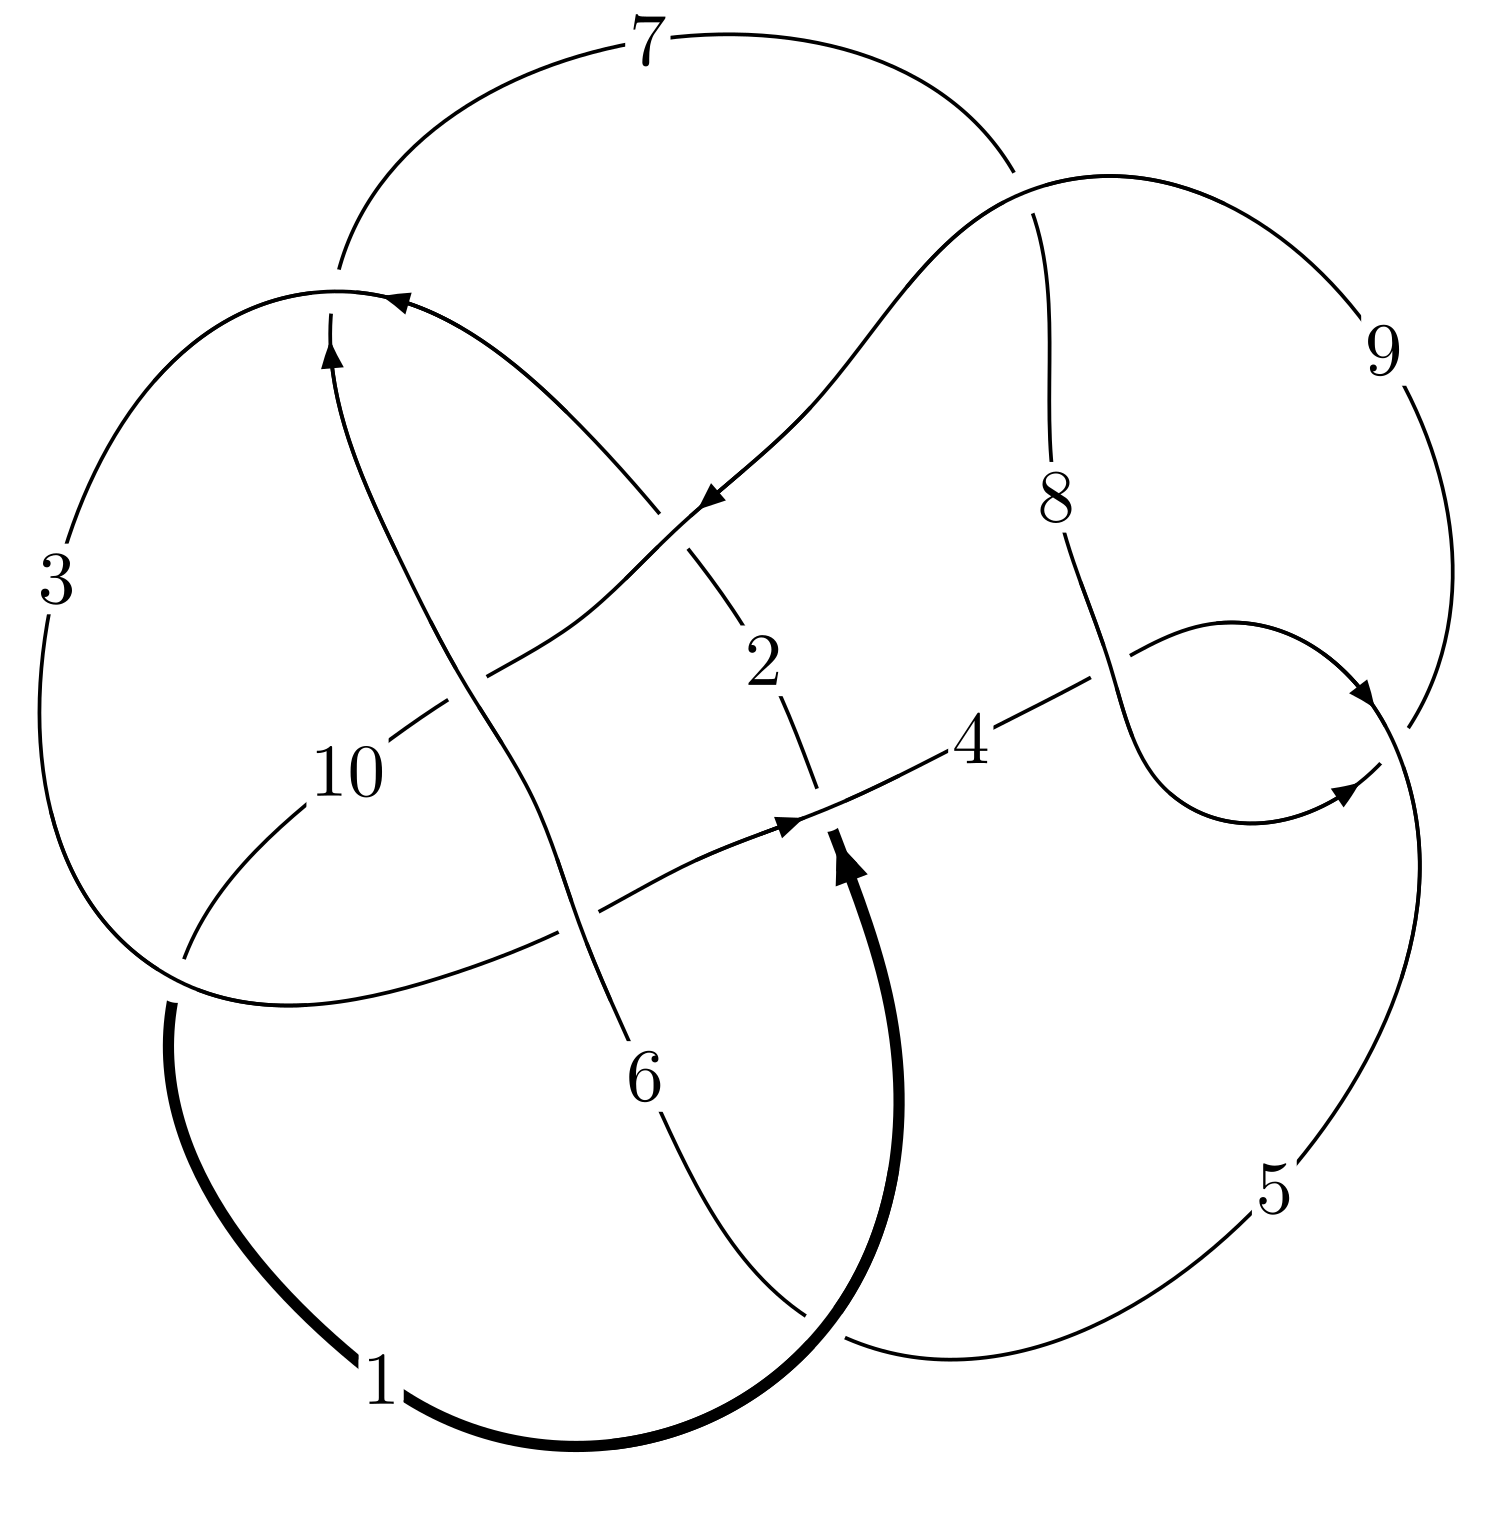
\includegraphics[width=112pt]{../../../GIT/diagram.site/Diagrams/png/231_10_147.png}\\
\ \ \ A knot diagram\footnotemark}&
\allowdisplaybreaks
\textbf{Linearized knot diagam} \\
\cline{2-2}
 &
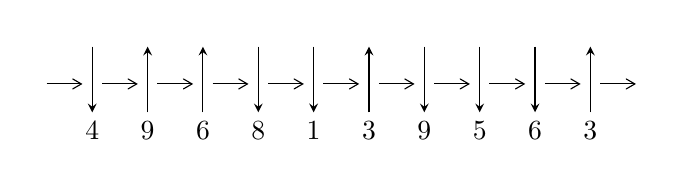
\begin{tikzpicture}[x=20pt, y=17pt]
	% nodes
	\node (C0) at (0, 0) {};
	\node (C1) at (1, 0) {};
	\node (C1U) at (1, +1) {};
	\node (C1D) at (1, -1) {4};

	\node (C2) at (2, 0) {};
	\node (C2U) at (2, +1) {};
	\node (C2D) at (2, -1) {9};

	\node (C3) at (3, 0) {};
	\node (C3U) at (3, +1) {};
	\node (C3D) at (3, -1) {6};

	\node (C4) at (4, 0) {};
	\node (C4U) at (4, +1) {};
	\node (C4D) at (4, -1) {8};

	\node (C5) at (5, 0) {};
	\node (C5U) at (5, +1) {};
	\node (C5D) at (5, -1) {1};

	\node (C6) at (6, 0) {};
	\node (C6U) at (6, +1) {};
	\node (C6D) at (6, -1) {3};

	\node (C7) at (7, 0) {};
	\node (C7U) at (7, +1) {};
	\node (C7D) at (7, -1) {9};

	\node (C8) at (8, 0) {};
	\node (C8U) at (8, +1) {};
	\node (C8D) at (8, -1) {5};

	\node (C9) at (9, 0) {};
	\node (C9U) at (9, +1) {};
	\node (C9D) at (9, -1) {6};

	\node (C10) at (10, 0) {};
	\node (C10U) at (10, +1) {};
	\node (C10D) at (10, -1) {3};
	\node (C11) at (11, 0) {};

	% arrows
	\draw[->,>={angle 60}]
	(C0) edge (C1) (C1) edge (C2) (C2) edge (C3) (C3) edge (C4) (C4) edge (C5) (C5) edge (C6) (C6) edge (C7) (C7) edge (C8) (C8) edge (C9) (C9) edge (C10) (C10) edge (C11) ;	\draw[->,>=stealth]
	(C1U) edge (C1D) (C2D) edge (C2U) (C3D) edge (C3U) (C4U) edge (C4D) (C5U) edge (C5D) (C6D) edge (C6U) (C7U) edge (C7D) (C8U) edge (C8D) (C9U) edge (C9D) (C10D) edge (C10U) ;
	\end{tikzpicture} \\
\hhline{~~} \\& 
\textbf{Solving Sequence} \\ \cline{2-2} 
 &
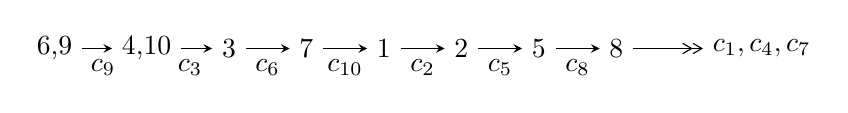
\begin{tikzpicture}[x=28pt, y=7pt]
	% node
	\node (A0) at (-1/8, 0) {6,9};
	\node (A1) at (17/16, 0) {4,10};
	\node (A2) at (17/8, 0) {3};
	\node (A3) at (25/8, 0) {7};
	\node (A4) at (33/8, 0) {1};
	\node (A5) at (41/8, 0) {2};
	\node (A6) at (49/8, 0) {5};
	\node (A7) at (57/8, 0) {8};
	\node (C1) at (1/2, -1) {$c_{9}$};
	\node (C2) at (13/8, -1) {$c_{3}$};
	\node (C3) at (21/8, -1) {$c_{6}$};
	\node (C4) at (29/8, -1) {$c_{10}$};
	\node (C5) at (37/8, -1) {$c_{2}$};
	\node (C6) at (45/8, -1) {$c_{5}$};
	\node (C7) at (53/8, -1) {$c_{8}$};
	\node (A8) at (9, 0) {$c_{1},c_{4},c_{7}$};

	% edge
	\draw[->,>=stealth]	
	(A0) edge (A1) (A1) edge (A2) (A2) edge (A3) (A3) edge (A4) (A4) edge (A5) (A5) edge (A6) (A6) edge (A7) ;
	\draw[->>,>={angle 60}]	
	(A7) edge (A8);
\end{tikzpicture} \\ 

\end{tabular} \\

\footnotetext{
The image of knot diagram is generated by the software ``\textbf{Draw programme}" developed by Andrew Bartholomew(\url{http://www.layer8.co.uk/maths/draw/index.htm\#Running-draw}), where we modified some parts for our purpose(\url{https://github.com/CATsTAILs/LinksPainter}).
}\phantom \\ \newline 
\centering \textbf{Ideals for irreducible components\footnotemark of $X_{\text{par}}$} 
 
\begin{align*}
I^u_{1}&=\langle 
713770382 u^{13}-2219758738 u^{12}+\cdots+3379396381 b+1752340181,\\
\phantom{I^u_{1}}&\phantom{= \langle  }-4583934274 u^{13}+15016790197 u^{12}+\cdots+3379396381 a+53453066,\;u^{14}-3 u^{13}+\cdots+6 u+1\rangle \\
I^u_{2}&=\langle 
- u^3- u^2+b-4 u-1,\;4 u^3+6 u^2+a+17 u+7,\;u^4+2 u^3+5 u^2+4 u+1\rangle \\
I^u_{3}&=\langle 
b,\;a-1,\;u^3+u+1\rangle \\
\\
\end{align*}
\raggedright * 3 irreducible components of $\dim_{\mathbb{C}}=0$, with total 21 representations.\\
\footnotetext{All coefficients of polynomials are rational numbers. But the coefficients are sometimes approximated in decimal forms when there is not enough margin.}
\newpage
\renewcommand{\arraystretch}{1}
\centering \section*{I. $I^u_{1}= \langle 7.14\times10^{8} u^{13}-2.22\times10^{9} u^{12}+\cdots+3.38\times10^{9} b+1.75\times10^{9},\;-4.58\times10^{9} u^{13}+1.50\times10^{10} u^{12}+\cdots+3.38\times10^{9} a+5.35\times10^{7},\;u^{14}-3 u^{13}+\cdots+6 u+1 \rangle$}
\flushleft \textbf{(i) Arc colorings}\\
\begin{tabular}{m{7pt} m{180pt} m{7pt} m{180pt} }
\flushright $a_{6}=$&$\begin{pmatrix}0\\u\end{pmatrix}$ \\
\flushright $a_{9}=$&$\begin{pmatrix}1\\0\end{pmatrix}$ \\
\flushright $a_{4}=$&$\begin{pmatrix}1.35644 u^{13}-4.44363 u^{12}+\cdots+29.0734 u-0.0158173\\-0.211212 u^{13}+0.656851 u^{12}+\cdots-7.55883 u-0.518536\end{pmatrix}$ \\
\flushright $a_{10}=$&$\begin{pmatrix}1\\u^2\end{pmatrix}$ \\
\flushright $a_{3}=$&$\begin{pmatrix}1.35644 u^{13}-4.44363 u^{12}+\cdots+29.0734 u-0.0158173\\-0.197062 u^{13}+0.657652 u^{12}+\cdots-6.66932 u-0.144213\end{pmatrix}$ \\
\flushright $a_{7}=$&$\begin{pmatrix}-0.664129 u^{13}+2.29385 u^{12}+\cdots-12.7349 u+5.55469\\0.0964891 u^{13}-0.391604 u^{12}+\cdots+1.77926 u-1.40855\end{pmatrix}$ \\
\flushright $a_{1}=$&$\begin{pmatrix}-1.10709 u^{13}+3.17567 u^{12}+\cdots-27.0789 u-7.56641\\0.194643 u^{13}-0.592457 u^{12}+\cdots+4.85079 u+1.66551\end{pmatrix}$ \\
\flushright $a_{2}=$&$\begin{pmatrix}1.55350 u^{13}-5.10128 u^{12}+\cdots+35.7427 u+0.128396\\-0.197062 u^{13}+0.657652 u^{12}+\cdots-6.66932 u-0.144213\end{pmatrix}$ \\
\flushright $a_{5}=$&$\begin{pmatrix}0.144213 u^{13}-0.629701 u^{12}+\cdots+3.65663 u-5.80404\\-0.0559147 u^{13}+0.229057 u^{12}+\cdots+0.863012 u+1.51536\end{pmatrix}$ \\
\flushright $a_{8}=$&$\begin{pmatrix}-0.760618 u^{13}+2.68545 u^{12}+\cdots-14.5142 u+6.96324\\0.0964891 u^{13}-0.391604 u^{12}+\cdots+1.77926 u-1.40855\end{pmatrix}$\\&\end{tabular}
\flushleft \textbf{(ii) Obstruction class $= -1$}\\~\\
\flushleft \textbf{(iii) Cusp Shapes $= -\frac{4583624542}{3379396381} u^{13}+\frac{13650120072}{3379396381} u^{12}+\cdots-\frac{173475920162}{3379396381} u-\frac{35870136224}{3379396381}$}\\~\\
\newpage\renewcommand{\arraystretch}{1}
\flushleft \textbf{(iv) u-Polynomials at the component}\newline \\
\begin{tabular}{m{50pt}|m{274pt}}
Crossings & \hspace{64pt}u-Polynomials at each crossing \\
\hline $$\begin{aligned}c_{1}\end{aligned}$$&$\begin{aligned}
&u^{14}-5 u^{13}+\cdots-32 u+29
\end{aligned}$\\
\hline $$\begin{aligned}c_{2}\end{aligned}$$&$\begin{aligned}
&u^{14}- u^{13}+\cdots+10 u+1
\end{aligned}$\\
\hline $$\begin{aligned}c_{3},c_{6}\end{aligned}$$&$\begin{aligned}
&u^{14}+u^{13}+\cdots-10 u+1
\end{aligned}$\\
\hline $$\begin{aligned}c_{4},c_{8}\end{aligned}$$&$\begin{aligned}
&u^{14}-2 u^{13}+\cdots-3 u+2
\end{aligned}$\\
\hline $$\begin{aligned}c_{5}\end{aligned}$$&$\begin{aligned}
&u^{14}+u^{13}+\cdots-4 u+1
\end{aligned}$\\
\hline $$\begin{aligned}c_{7}\end{aligned}$$&$\begin{aligned}
&u^{14}+8 u^{13}+\cdots-19 u+4
\end{aligned}$\\
\hline $$\begin{aligned}c_{9}\end{aligned}$$&$\begin{aligned}
&u^{14}-3 u^{13}+\cdots+6 u+1
\end{aligned}$\\
\hline $$\begin{aligned}c_{10}\end{aligned}$$&$\begin{aligned}
&u^{14}+3 u^{13}+\cdots+7 u+62
\end{aligned}$\\
\hline
\end{tabular}\\~\\
\newpage\renewcommand{\arraystretch}{1}
\flushleft \textbf{(v) Riley Polynomials at the component}\newline \\
\begin{tabular}{m{50pt}|m{274pt}}
Crossings & \hspace{64pt}Riley Polynomials at each crossing \\
\hline $$\begin{aligned}c_{1}\end{aligned}$$&$\begin{aligned}
&y^{14}-17 y^{13}+\cdots-3924 y+841
\end{aligned}$\\
\hline $$\begin{aligned}c_{2}\end{aligned}$$&$\begin{aligned}
&y^{14}+29 y^{13}+\cdots-54 y+1
\end{aligned}$\\
\hline $$\begin{aligned}c_{3},c_{6}\end{aligned}$$&$\begin{aligned}
&y^{14}+21 y^{13}+\cdots-42 y+1
\end{aligned}$\\
\hline $$\begin{aligned}c_{4},c_{8}\end{aligned}$$&$\begin{aligned}
&y^{14}-8 y^{13}+\cdots+19 y+4
\end{aligned}$\\
\hline $$\begin{aligned}c_{5}\end{aligned}$$&$\begin{aligned}
&y^{14}+y^{13}+\cdots-10 y+1
\end{aligned}$\\
\hline $$\begin{aligned}c_{7}\end{aligned}$$&$\begin{aligned}
&y^{14}-4 y^{13}+\cdots-417 y+16
\end{aligned}$\\
\hline $$\begin{aligned}c_{9}\end{aligned}$$&$\begin{aligned}
&y^{14}-33 y^{13}+\cdots+36 y+1
\end{aligned}$\\
\hline $$\begin{aligned}c_{10}\end{aligned}$$&$\begin{aligned}
&y^{14}+25 y^{13}+\cdots+20163 y+3844
\end{aligned}$\\
\hline
\end{tabular}\\~\\
\newpage\flushleft \textbf{(vi) Complex Volumes and Cusp Shapes}
$$\begin{array}{c|c|c}  
\text{Solutions to }I^u_{1}& \I (\text{vol} + \sqrt{-1}CS) & \text{Cusp shape}\\
 \hline 
\begin{aligned}
u &= -0.237387 + 0.876423 I \\
a &= \phantom{-}0.004721 - 0.208169 I \\
b &= -0.869563 - 0.338885 I\end{aligned}
 & \phantom{-}1.74438 + 2.05841 I & \phantom{-}4.16985 - 4.09365 I \\ \hline\begin{aligned}
u &= -0.237387 - 0.876423 I \\
a &= \phantom{-}0.004721 + 0.208169 I \\
b &= -0.869563 + 0.338885 I\end{aligned}
 & \phantom{-}1.74438 - 2.05841 I & \phantom{-}4.16985 + 4.09365 I \\ \hline\begin{aligned}
u &= -0.595439 + 0.915402 I \\
a &= \phantom{-}0.915640 - 0.422475 I \\
b &= \phantom{-}1.027050 + 0.729987 I\end{aligned}
 & -1.83211 + 2.08733 I & -7.27574 - 2.80711 I \\ \hline\begin{aligned}
u &= -0.595439 - 0.915402 I \\
a &= \phantom{-}0.915640 + 0.422475 I \\
b &= \phantom{-}1.027050 - 0.729987 I\end{aligned}
 & -1.83211 - 2.08733 I & -7.27574 + 2.80711 I \\ \hline\begin{aligned}
u &= \phantom{-}0.021578 + 0.347833 I \\
a &= \phantom{-}1.92553 - 1.06606 I \\
b &= \phantom{-}0.029013 - 0.667088 I\end{aligned}
 & -0.11203 + 1.46789 I & -1.17938 - 4.69179 I \\ \hline\begin{aligned}
u &= \phantom{-}0.021578 - 0.347833 I \\
a &= \phantom{-}1.92553 + 1.06606 I \\
b &= \phantom{-}0.029013 + 0.667088 I\end{aligned}
 & -0.11203 - 1.46789 I & -1.17938 + 4.69179 I \\ \hline\begin{aligned}
u &= -0.113601 + 0.166050 I \\
a &= -1.16417 + 5.61112 I \\
b &= \phantom{-}0.064203 - 1.109710 I\end{aligned}
 & -3.57417 + 4.92202 I & -5.84899 - 5.58919 I \\ \hline\begin{aligned}
u &= -0.113601 - 0.166050 I \\
a &= -1.16417 - 5.61112 I \\
b &= \phantom{-}0.064203 + 1.109710 I\end{aligned}
 & -3.57417 - 4.92202 I & -5.84899 + 5.58919 I \\ \hline\begin{aligned}
u &= \phantom{-}2.25002 + 0.12421 I \\
a &= -0.037619 - 0.804931 I \\
b &= \phantom{-}0.43823 + 1.90805 I\end{aligned}
 & -13.29020 - 1.42119 I & -6.81603 + 0.70499 I \\ \hline\begin{aligned}
u &= \phantom{-}2.25002 - 0.12421 I \\
a &= -0.037619 + 0.804931 I \\
b &= \phantom{-}0.43823 - 1.90805 I\end{aligned}
 & -13.29020 + 1.42119 I & -6.81603 - 0.70499 I\\
 \hline 
 \end{array}$$\newpage$$\begin{array}{c|c|c}  
\text{Solutions to }I^u_{1}& \I (\text{vol} + \sqrt{-1}CS) & \text{Cusp shape}\\
 \hline 
\begin{aligned}
u &= -2.43987 + 0.07821 I \\
a &= -0.036182 - 0.696454 I \\
b &= \phantom{-}0.47053 + 2.07372 I\end{aligned}
 & -8.54619 + 3.71322 I & -3.42485 - 2.09291 I \\ \hline\begin{aligned}
u &= -2.43987 - 0.07821 I \\
a &= -0.036182 + 0.696454 I \\
b &= \phantom{-}0.47053 - 2.07372 I\end{aligned}
 & -8.54619 - 3.71322 I & -3.42485 + 2.09291 I \\ \hline\begin{aligned}
u &= \phantom{-}2.61470 + 0.01753 I \\
a &= -0.107927 + 0.663193 I \\
b &= \phantom{-}0.34053 - 2.14014 I\end{aligned}
 & -12.2232 - 9.4176 I & -5.62486 + 4.99855 I \\ \hline\begin{aligned}
u &= \phantom{-}2.61470 - 0.01753 I \\
a &= -0.107927 - 0.663193 I \\
b &= \phantom{-}0.34053 + 2.14014 I\end{aligned}
 & -12.2232 + 9.4176 I & -5.62486 - 4.99855 I\\
 \hline 
 \end{array}$$\newpage\newpage\renewcommand{\arraystretch}{1}
\centering \section*{II. $I^u_{2}= \langle - u^3- u^2+b-4 u-1,\;4 u^3+6 u^2+a+17 u+7,\;u^4+2 u^3+5 u^2+4 u+1 \rangle$}
\flushleft \textbf{(i) Arc colorings}\\
\begin{tabular}{m{7pt} m{180pt} m{7pt} m{180pt} }
\flushright $a_{6}=$&$\begin{pmatrix}0\\u\end{pmatrix}$ \\
\flushright $a_{9}=$&$\begin{pmatrix}1\\0\end{pmatrix}$ \\
\flushright $a_{4}=$&$\begin{pmatrix}-4 u^3-6 u^2-17 u-7\\u^3+u^2+4 u+1\end{pmatrix}$ \\
\flushright $a_{10}=$&$\begin{pmatrix}1\\u^2\end{pmatrix}$ \\
\flushright $a_{3}=$&$\begin{pmatrix}-4 u^3-6 u^2-17 u-7\\-1\end{pmatrix}$ \\
\flushright $a_{7}=$&$\begin{pmatrix}u^3+2 u^2+5 u+4\\-2 u^3-3 u^2-8 u-4\end{pmatrix}$ \\
\flushright $a_{1}=$&$\begin{pmatrix}-4 u^3-6 u^2-17 u-7\\u^3+2 u^2+4 u+1\end{pmatrix}$ \\
\flushright $a_{2}=$&$\begin{pmatrix}-4 u^3-6 u^2-17 u-6\\-1\end{pmatrix}$ \\
\flushright $a_{5}=$&$\begin{pmatrix}u^3+2 u^2+5 u+4\\- u^3-2 u^2-5 u-3\end{pmatrix}$ \\
\flushright $a_{8}=$&$\begin{pmatrix}3 u^3+5 u^2+13 u+8\\-2 u^3-3 u^2-8 u-4\end{pmatrix}$\\&\end{tabular}
\flushleft \textbf{(ii) Obstruction class $= 1$}\\~\\
\flushleft \textbf{(iii) Cusp Shapes $= 8 u^3+12 u^2+32 u+12$}\\~\\
\newpage\renewcommand{\arraystretch}{1}
\flushleft \textbf{(iv) u-Polynomials at the component}\newline \\
\begin{tabular}{m{50pt}|m{274pt}}
Crossings & \hspace{64pt}u-Polynomials at each crossing \\
\hline $$\begin{aligned}c_{1}\end{aligned}$$&$\begin{aligned}
&u^4-4 u^3+5 u^2-2 u+1
\end{aligned}$\\
\hline $$\begin{aligned}c_{2}\end{aligned}$$&$\begin{aligned}
&(u-1)^4
\end{aligned}$\\
\hline $$\begin{aligned}c_{3},c_{5},c_{6}\end{aligned}$$&$\begin{aligned}
&(u^2+1)^2
\end{aligned}$\\
\hline $$\begin{aligned}c_{4},c_{8},c_{10}\end{aligned}$$&$\begin{aligned}
&u^4- u^2+1
\end{aligned}$\\
\hline $$\begin{aligned}c_{7}\end{aligned}$$&$\begin{aligned}
&(u^2- u+1)^2
\end{aligned}$\\
\hline $$\begin{aligned}c_{9}\end{aligned}$$&$\begin{aligned}
&u^4+2 u^3+5 u^2+4 u+1
\end{aligned}$\\
\hline
\end{tabular}\\~\\
\newpage\renewcommand{\arraystretch}{1}
\flushleft \textbf{(v) Riley Polynomials at the component}\newline \\
\begin{tabular}{m{50pt}|m{274pt}}
Crossings & \hspace{64pt}Riley Polynomials at each crossing \\
\hline $$\begin{aligned}c_{1}\end{aligned}$$&$\begin{aligned}
&y^4-6 y^3+11 y^2+6 y+1
\end{aligned}$\\
\hline $$\begin{aligned}c_{2}\end{aligned}$$&$\begin{aligned}
&(y-1)^4
\end{aligned}$\\
\hline $$\begin{aligned}c_{3},c_{5},c_{6}\end{aligned}$$&$\begin{aligned}
&(y+1)^4
\end{aligned}$\\
\hline $$\begin{aligned}c_{4},c_{8},c_{10}\end{aligned}$$&$\begin{aligned}
&(y^2- y+1)^2
\end{aligned}$\\
\hline $$\begin{aligned}c_{7}\end{aligned}$$&$\begin{aligned}
&(y^2+y+1)^2
\end{aligned}$\\
\hline $$\begin{aligned}c_{9}\end{aligned}$$&$\begin{aligned}
&y^4+6 y^3+11 y^2-6 y+1
\end{aligned}$\\
\hline
\end{tabular}\\~\\
\newpage\flushleft \textbf{(vi) Complex Volumes and Cusp Shapes}
$$\begin{array}{c|c|c}  
\text{Solutions to }I^u_{2}& \I (\text{vol} + \sqrt{-1}CS) & \text{Cusp shape}\\
 \hline 
\begin{aligned}
u &= -0.500000 + 0.133975 I \\
a &= \phantom{-}0.50000 - 1.86603 I \\
b &= -0.866025 + 0.500000 I\end{aligned}
 & \phantom{-0.000000 } -2.02988 I & -2.00000 + 3.46410 I \\ \hline\begin{aligned}
u &= -0.500000 - 0.133975 I \\
a &= \phantom{-}0.50000 + 1.86603 I \\
b &= -0.866025 - 0.500000 I\end{aligned}
 & \phantom{-0.000000 -}2.02988 I & -2.00000 - 3.46410 I \\ \hline\begin{aligned}
u &= -0.50000 + 1.86603 I \\
a &= \phantom{-}0.500000 - 0.133975 I \\
b &= \phantom{-}0.866025 + 0.500000 I\end{aligned}
 & \phantom{-0.000000 -}2.02988 I & -2.00000 - 3.46410 I \\ \hline\begin{aligned}
u &= -0.50000 - 1.86603 I \\
a &= \phantom{-}0.500000 + 0.133975 I \\
b &= \phantom{-}0.866025 - 0.500000 I\end{aligned}
 & \phantom{-0.000000 } -2.02988 I & -2.00000 + 3.46410 I\\
 \hline 
 \end{array}$$\newpage\newpage\renewcommand{\arraystretch}{1}
\centering \section*{III. $I^u_{3}= \langle b,\;a-1,\;u^3+u+1 \rangle$}
\flushleft \textbf{(i) Arc colorings}\\
\begin{tabular}{m{7pt} m{180pt} m{7pt} m{180pt} }
\flushright $a_{6}=$&$\begin{pmatrix}0\\u\end{pmatrix}$ \\
\flushright $a_{9}=$&$\begin{pmatrix}1\\0\end{pmatrix}$ \\
\flushright $a_{4}=$&$\begin{pmatrix}1\\0\end{pmatrix}$ \\
\flushright $a_{10}=$&$\begin{pmatrix}1\\u^2\end{pmatrix}$ \\
\flushright $a_{3}=$&$\begin{pmatrix}1\\u^2\end{pmatrix}$ \\
\flushright $a_{7}=$&$\begin{pmatrix}u\\-1\end{pmatrix}$ \\
\flushright $a_{1}=$&$\begin{pmatrix}1\\u^2\end{pmatrix}$ \\
\flushright $a_{2}=$&$\begin{pmatrix}- u^2+1\\u^2\end{pmatrix}$ \\
\flushright $a_{5}=$&$\begin{pmatrix}u\\-1\end{pmatrix}$ \\
\flushright $a_{8}=$&$\begin{pmatrix}u+1\\-1\end{pmatrix}$\\&\end{tabular}
\flushleft \textbf{(ii) Obstruction class $= -1$}\\~\\
\flushleft \textbf{(iii) Cusp Shapes $= -6$}\\~\\
\newpage\renewcommand{\arraystretch}{1}
\flushleft \textbf{(iv) u-Polynomials at the component}\newline \\
\begin{tabular}{m{50pt}|m{274pt}}
Crossings & \hspace{64pt}u-Polynomials at each crossing \\
\hline $$\begin{aligned}c_{1}\end{aligned}$$&$\begin{aligned}
&u^3+2 u^2+u-1
\end{aligned}$\\
\hline $$\begin{aligned}c_{2}\end{aligned}$$&$\begin{aligned}
&u^3-2 u^2+u+1
\end{aligned}$\\
\hline $$\begin{aligned}c_{3},c_{5},c_{6}\\c_{9}\end{aligned}$$&$\begin{aligned}
&u^3+u+1
\end{aligned}$\\
\hline $$\begin{aligned}c_{4},c_{7},c_{8}\end{aligned}$$&$\begin{aligned}
&(u+1)^3
\end{aligned}$\\
\hline $$\begin{aligned}c_{10}\end{aligned}$$&$\begin{aligned}
&u^3
\end{aligned}$\\
\hline
\end{tabular}\\~\\
\newpage\renewcommand{\arraystretch}{1}
\flushleft \textbf{(v) Riley Polynomials at the component}\newline \\
\begin{tabular}{m{50pt}|m{274pt}}
Crossings & \hspace{64pt}Riley Polynomials at each crossing \\
\hline $$\begin{aligned}c_{1},c_{2}\end{aligned}$$&$\begin{aligned}
&y^3-2 y^2+5 y-1
\end{aligned}$\\
\hline $$\begin{aligned}c_{3},c_{5},c_{6}\\c_{9}\end{aligned}$$&$\begin{aligned}
&y^3+2 y^2+y-1
\end{aligned}$\\
\hline $$\begin{aligned}c_{4},c_{7},c_{8}\end{aligned}$$&$\begin{aligned}
&(y-1)^3
\end{aligned}$\\
\hline $$\begin{aligned}c_{10}\end{aligned}$$&$\begin{aligned}
&y^3
\end{aligned}$\\
\hline
\end{tabular}\\~\\
\newpage\flushleft \textbf{(vi) Complex Volumes and Cusp Shapes}
$$\begin{array}{c|c|c}  
\text{Solutions to }I^u_{3}& \I (\text{vol} + \sqrt{-1}CS) & \text{Cusp shape}\\
 \hline 
\begin{aligned}
u &= \phantom{-}0.341164 + 1.161540 I \\
a &= \phantom{-}1.00000\phantom{ +0.000000I} \\
b &= \phantom{-0.000000 } 0\end{aligned}
 & -1.64493\phantom{ +0.000000I} & -6.00000\phantom{ +0.000000I} \\ \hline\begin{aligned}
u &= \phantom{-}0.341164 - 1.161540 I \\
a &= \phantom{-}1.00000\phantom{ +0.000000I} \\
b &= \phantom{-0.000000 } 0\end{aligned}
 & -1.64493\phantom{ +0.000000I} & -6.00000\phantom{ +0.000000I} \\ \hline\begin{aligned}
u &= -0.682328\phantom{ +0.000000I} \\
a &= \phantom{-}1.00000\phantom{ +0.000000I} \\
b &= \phantom{-0.000000 } 0\end{aligned}
 & -1.64493\phantom{ +0.000000I} & -6.00000\phantom{ +0.000000I}\\
 \hline 
 \end{array}$$\newpage
\newpage\renewcommand{\arraystretch}{1}
\centering \section*{ IV. u-Polynomials}
\begin{tabular}{m{50pt}|m{274pt}}
Crossings & \hspace{64pt}u-Polynomials at each crossing \\
\hline $$\begin{aligned}c_{1}\end{aligned}$$&$\begin{aligned}
&(u^3+2 u^2+u-1)(u^4-4 u^3+\cdots-2 u+1)(u^{14}-5 u^{13}+\cdots-32 u+29)
\end{aligned}$\\
\hline $$\begin{aligned}c_{2}\end{aligned}$$&$\begin{aligned}
&((u-1)^4)(u^3-2 u^2+u+1)(u^{14}- u^{13}+\cdots+10 u+1)
\end{aligned}$\\
\hline $$\begin{aligned}c_{3},c_{6}\end{aligned}$$&$\begin{aligned}
&((u^2+1)^2)(u^3+u+1)(u^{14}+u^{13}+\cdots-10 u+1)
\end{aligned}$\\
\hline $$\begin{aligned}c_{4},c_{8}\end{aligned}$$&$\begin{aligned}
&((u+1)^3)(u^4- u^2+1)(u^{14}-2 u^{13}+\cdots-3 u+2)
\end{aligned}$\\
\hline $$\begin{aligned}c_{5}\end{aligned}$$&$\begin{aligned}
&((u^2+1)^2)(u^3+u+1)(u^{14}+u^{13}+\cdots-4 u+1)
\end{aligned}$\\
\hline $$\begin{aligned}c_{7}\end{aligned}$$&$\begin{aligned}
&((u+1)^3)(u^2- u+1)^2(u^{14}+8 u^{13}+\cdots-19 u+4)
\end{aligned}$\\
\hline $$\begin{aligned}c_{9}\end{aligned}$$&$\begin{aligned}
&(u^3+u+1)(u^4+2 u^3+\cdots+4 u+1)(u^{14}-3 u^{13}+\cdots+6 u+1)
\end{aligned}$\\
\hline $$\begin{aligned}c_{10}\end{aligned}$$&$\begin{aligned}
&u^3(u^4- u^2+1)(u^{14}+3 u^{13}+\cdots+7 u+62)
\end{aligned}$\\
\hline
\end{tabular}\newpage\renewcommand{\arraystretch}{1}
\centering \section*{ V. Riley Polynomials}
\begin{tabular}{m{50pt}|m{274pt}}
Crossings & \hspace{64pt}Riley Polynomials at each crossing \\
\hline $$\begin{aligned}c_{1}\end{aligned}$$&$\begin{aligned}
&(y^3-2 y^2+5 y-1)(y^4-6 y^3+11 y^2+6 y+1)\\
&\cdot(y^{14}-17 y^{13}+\cdots-3924 y+841)
\end{aligned}$\\
\hline $$\begin{aligned}c_{2}\end{aligned}$$&$\begin{aligned}
&((y-1)^4)(y^3-2 y^2+5 y-1)(y^{14}+29 y^{13}+\cdots-54 y+1)
\end{aligned}$\\
\hline $$\begin{aligned}c_{3},c_{6}\end{aligned}$$&$\begin{aligned}
&((y+1)^4)(y^3+2 y^2+y-1)(y^{14}+21 y^{13}+\cdots-42 y+1)
\end{aligned}$\\
\hline $$\begin{aligned}c_{4},c_{8}\end{aligned}$$&$\begin{aligned}
&((y-1)^3)(y^2- y+1)^2(y^{14}-8 y^{13}+\cdots+19 y+4)
\end{aligned}$\\
\hline $$\begin{aligned}c_{5}\end{aligned}$$&$\begin{aligned}
&((y+1)^4)(y^3+2 y^2+y-1)(y^{14}+y^{13}+\cdots-10 y+1)
\end{aligned}$\\
\hline $$\begin{aligned}c_{7}\end{aligned}$$&$\begin{aligned}
&((y-1)^3)(y^2+y+1)^2(y^{14}-4 y^{13}+\cdots-417 y+16)
\end{aligned}$\\
\hline $$\begin{aligned}c_{9}\end{aligned}$$&$\begin{aligned}
&(y^3+2 y^2+y-1)(y^4+6 y^3+\cdots-6 y+1)(y^{14}-33 y^{13}+\cdots+36 y+1)
\end{aligned}$\\
\hline $$\begin{aligned}c_{10}\end{aligned}$$&$\begin{aligned}
&y^3(y^2- y+1)^2(y^{14}+25 y^{13}+\cdots+20163 y+3844)
\end{aligned}$\\
\hline
\end{tabular}
\vskip 2pc
\end{document}